\section*{Нестандартные функции потерь. Метод наименьших модулей. Квант\'{и}льная регрессия.}

Квадратичная функция потерь обычно дает хорошие результаты, является удобной в использовании, а потому и применяется чаще всего. Но в некоторых ситуациях она все же неприменима, и приходится использовать нестандартные функции потерь.

\subsection*{Метод наименьших модулей.}

Здесь и далее будем использовать следующие обозначения: $\ell$ - количество объектов в тренировочной выборке, $x_i$ ($i \in \left\{1, \dotsc, \ell \right\}$) - вектор признаков, $y_i$ ($i \in \left\{1, \dotsc, \ell \right\}$) - таргет, $a$ - модель, $\varepsilon_i := a(x_i) - y_i$ ($i \in \left\{1, \dotsc, \ell \right\}$).

Для стандартной квадратичной функции потерь $\mathscr{L}(\varepsilon) = \varepsilon^2$ задача будет выглядеть так:
$$\frac{1}{\ell}\sum\limits_{i=1}^\ell\left(a(x_i) - y_i\right)^2 \longrightarrow \min\limits_{a}.$$

Заменим функцию потерь на $\mathscr{L}(\varepsilon) = |\varepsilon|$.
Задача станет выглядеть так:
$$\frac{1}{\ell}\sum\limits_{i=1}^\ell\left|a(x_i) - y_i\right| \longrightarrow \min\limits_{a}.$$
Данный метод называется \textit{методом наименьших модулей}.

В какой ситуации такой подход может оказаться полезным? Рассмотрим ситуацию,  когда наша модель - это константа, то есть она вообще не зависит от признаков. Для квадратичной функции потерь получим:
$$\frac{1}{\ell}\sum\limits_{i=1}^\ell\left(a - y_i\right)^2 \longrightarrow \min\limits_{a}.$$
Здесь можно посчитать ответ аналитически, оптимальной константой $a$ будет $a = \frac{1}{\ell}\sum\limits_{i=1}^\ell y_i$, то есть среднее арифметическое таргетов. Это плохая оценка, если, например, в нашей выборке присутствуют выбросы, или распределение ошибок имеет тяжёлые <<хвосты>>.

А в случае использования метода наименьших модулей задача будет выглядеть так:
$$\frac{1}{\ell}\sum\limits_{i=1}^\ell\left|a - y_i\right| \longrightarrow \min\limits_{a}.$$
Здесь опять же можно посчитать ответ аналитически, оптимальным $a$ будет $a = \text{median}\left\{ y_1, \dotsc, y_\ell \right\} = y_{(\ell / 2)}$ (серединный член вариационного ряда). Эта оценка хороша тем, что устойчива к выбросам, хорошо работает для распределений ошибок с тяжелыми <<хвостами>>.

Таким образом, использование метода наименьших модулей в некоторых ситуациях помогает бороться с выбросами.

\subsection*{Квант\'{и}льная регрессия.}

Метод наименьших модулей можно обобщить. Давайте по-разному штрафовать отрицательные и положительные ошибки. Т.е. будем рассматривать функцию потерь вида
$$\mathscr{L}(\varepsilon) = \begin{cases}
    C_+|\varepsilon|, \varepsilon \geq 0,\\
    C_-|\varepsilon|, \varepsilon < 0.
\end{cases}$$

\begin{figure}[h]
    \centering
    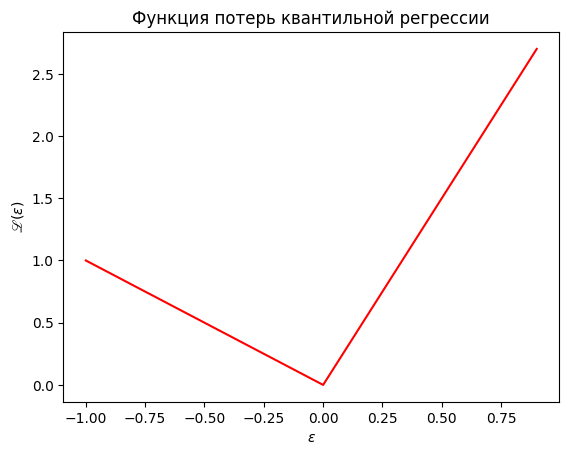
\includegraphics{chapters/nonstandart_error/images/ФПКР.png}
\end{figure}

Опять же рассмотрим случай, когда модель не зависит от признаков, то есть является константой:
$$\frac{1}{\ell}\sum\limits_{i=1}^\ell\mathscr{L}\left(a - y_i\right) \longrightarrow \min\limits_{a}.$$
Решение данной задачи опять же можно получить аналитически, оптимальным $a$ будет $a = y_{(q)}$ ($q$-тый член вариационного ряда), где $q = \frac{\ell C_-}{C_- + C_+}$.
Именно поэтому используемый метод называется \textit{методом квант\'{и}льной регрессии}.

Рассмотрим также еще один случай, когда квантильная регрессия оказывается хорошим вариантом с точки зрения решения задачи оптимизации, а именно случай линейной модели: $a(x) = \left\langle x, w \right\rangle$, где $w$ - вектор весов.

Сделаем замену переменных $\varepsilon_i^+ = (a(x_i) - y_i)_+$, $\varepsilon_i^- = (a(x_i) - y_i)_-$. Тогда наша задача будет иметь вид
$$\begin{cases}
    \frac{1}{\ell}\sum_{i=1}^\ell C_+\varepsilon_i^+ + C_-\varepsilon_i^- \longrightarrow \min\limits_{w},\\
    \left\langle w, x_i \right\rangle - y_i = \varepsilon_i^+ - \varepsilon_i^-, i \in \left\{ 1 , \dotsc, \ell \right\}.
\end{cases}$$

Это задача линейного программирования, для решения которой существует масса способов.

\newpage

\subsection*{Задачи.}

\subsubsection*{Задача 1.}

Предположим, у Вас есть датасет с данными о жителях некоторой страны Южной или Центральной Африки, а также данные об их среднем ежедневном доходе, и Вы хотите научиться предсказывать этот доход по значениям рассматриваемых признаков. Полученная модель в последующем будет использоваться для составления плана по оказанию гуманитарной помощи населению. Что использовать предпочтительнее: квадратичную функцию потерь или функцию потерь квант\'{и}льной регрессии? Почему? Если использовать предпочтительнее функцию потерь квант\'{и}льной регрессии, то каким должно быть соотношение параметров $C_+$ и $C_-$ и почему?

\begin{solution}
    В условии задачи не зря указано, из какого региона у нас страна. Б\'{о}льшая часть населения в ней, скорее всего, крайне бедна, при этом есть очень незначительное количество сверхбогатых людей, т.е., в нашей терминологии, выбросов. Поэтому функция потерь квант\'{и}льной регрессии более предпочтительна, чем квадратичная функция потерь.

    Теперь обратим внимание на то, как будет использована модель, чтобы понять, какая ошибка для нас наиболее страшна: положительная или отрицательная. Заметим, что если мы предсказали доход человека больше реального, т.е. ошибка положительна, то, скорее всего, на него будет выделено меньше помощи. Это кажется более страшным, чем ситуация, в которой мы предсказали доход человека меньше реального, и дали ему чуть больше помощи. Поэтому штрафовать положительные ошибки стоит сильнее, чем отрицательные, то есть стоит выбрать $C_+$ и $C_-$ так, чтобы $C_+/C_- > 1$.
\end{solution}

\subsubsection*{Задача 2.}

Предположим, что у в природе некоторый таргет действительно линейно зависит от вектора признаков, но вектор таргетов, который у нас есть, зашумлен ошбиками, причем ошибки эти приходят из симметричного распределения Коши. Почему использование квадратичной функции потерь в данном случае будет крайне нежелательным? А если ошибки приходит из распределения $\mathcal{N}(a, \sigma^2)$, где $a \neq 0$?

\begin{solution}
    Из теории вероятностей и математической статистики известно, что у распределения Коши тяжелые <<хвосты>>, из-за чего у него даже нет матожидания. Именно поэтому квадратичная функция потерь, очень сильно штрафующая за большие ошибки, здесь не подходит. А вот метод наименьших модулей подхолит лучше.

    Также можно заметить, что квадратичная функция потерь одинаково штрафует положительные и отрицательные ошибки, то есть неявно подразумевается симметричность распределения. В общем случае это не так. Квант\'{и}льная регрессия позволяет более гибко работать с несимметричными распределениями.
\end{solution}

\subsubsection*{Задача 3.}

Предположим, что Вы тестируете новое лекарство на мышах. Вы хотите понять, какая доза лекарства оптимальна: уже вылечивает мышь, но все еще не дает негативных побочных эффектов. Известно, что каждый новый побочный эффект проявляется при превышении некоторого примерно одинакового для всех мышей порога передозировки и действует все сильнее и сильнее при дальнейшем превышении этого порога. Также известно, что оптимум не единственен, а достигается на некотором отрезке, длина которого вам тоже заранее известна. Наконец, ниже некоторого порога лекарство действует все хуже и хуже. У Вас есть некоторые данные о мышах, а также таргеты - максимальные оптимальные дозы лекарств. Предложите модификацию функции потерь квант\'{и}льной регрессии, оптимальную для данной задачи.

\begin{solution}
    Основная идея квант\'{и}льной регрессии по сравнению с методом наименьших модулей состоит в том, что мы по-разному штрафуем положительные и отрицательные ошибки. Давайте разовьем эту идею, и будем по-разному штрафовать ошибки в зависимости от того, в какую часть числовой прямой мы попали.

    Так, для нашей задачи, пусть новые побочные эффекты проявляются при превышении дозировки на $a_1, \dotsc, a_n$ у.е., где $0= a_1 < \ldots < a_n$. А длина оптимального отрезка дозировки равна $b$, Тогда можно взять такую функцию потерь:
    $$\mathscr{L}(\varepsilon) = \begin{cases}
        -v_b\varepsilon, \varepsilon < -b,\\
        0, \varepsilon \in [-b; a_1],\\
        v_{a_1}\varepsilon, \varepsilon \in (a_1; a_2],\\
        (v_{a_1} + v_{a_2})\varepsilon, \varepsilon \in (a_2; a_3],\\
        \vdots\\
        (v_{a_1} + \dotsb + v_{a_{n - 1}})\varepsilon, \varepsilon \in (a_{n-1}; a_n],\\
        (v_{a_1} + \dotsb + v_{a_n})\varepsilon, \varepsilon > a_n,
    \end{cases}$$
    где $v_b, v_{a_1}, \dotsc, v_{a_n}$ - скорости роста соответствующих проблем.
\end{solution}

\newpage
\section*{SVM-Regression}

Регрессионные модели на основе метода опорных векторов (SVM-regression) зачастую используют особую функцию потерь, отличающуюся от стандартной квадратичной ошибки (MSE). В частности, классический SVM для регрессии использует \(\varepsilon\)-insensitive функцию потерь (\(\varepsilon\)-insensitive loss), которая игнорирует ошибки, величина которых меньше заранее заданного порога \(\varepsilon\). Однако существуют и нестандартные функции потерь, которые могут быть полезны в специфических задачах, например, когда необходимо учитывать асимметрию ошибок, различные веса отдельных наблюдений или же более сложные, ориентированные на распределение отклонений, формулы.

Классическая \(\varepsilon\)-insensitive функция потерь:
Для модели вида \(f(x) = \langle w, x \rangle + b\) функция потерь определяется следующим образом:
\begin{align*}
L(\varepsilon) = \max(0, | y - f(x) | - \varepsilon).
\end{align*}

Если \(| y - f(x) | \leq \varepsilon\), то штраф равен нулю, что делает модель нечувствительной к небольшим отклонениям и позволяет контролировать сложность аппроксимации.

Нестандартные функции потерь могут иметь следующие особенности:

\begin{enumerate}
    \item Асимметричные функции потерь: например, более сильное штрафование положительных отклонений, чем отрицательных, или наоборот. Это может быть полезно, если цена переоценки или недооценки целевой переменной различна.
    \item Частично-кусочные функции: использование различных режимов штрафования в зависимости от величины отклонения, например, линейная область штрафа для малых ошибок и квадратичная — для больших.
    \item Функции с весами для разных точек: если некоторые точки обучающей выборки важнее, можно ввести веса и штрафовать ошибки по более значимым точкам сильнее.
    \item Нелинейные преобразования ошибки: например, логарифмическая или экспоненциальная функция потерь, которая меняет чувствительность модели к большим отклонениям.
\end{enumerate}

Пример асимметричной \(\varepsilon\)-insensitive функции потерь:
\begin{align*}
    L(\varepsilon, \alpha) = 
        \begin{cases}
            0, & | y - f(x) | \leq \varepsilon \\
            \alpha(y - f(x)) - \varepsilon, & y - f(x) > \varepsilon \\
            \frac{(y - f(x))}{\alpha} - \varepsilon, & f(x) - y > \varepsilon
        \end{cases}
\end{align*}
где \(\alpha > 1\) задаёт степень асимметрии штрафования. Такая функция потерь позволит модели сильнее реагировать на недостаточную оценку и слабее —-- на переоценку.

\newpage
\subsection*{Задачи}

\subsubsection*{Задача 1.}
Пусть у нас есть набор точек для регрессии \(\{(x_i, y_i)\}_{i=1}^m\), и используется \(\varepsilon\)-insensitive функция потерь. Как будет влиять на итоговую модель выбор \(\varepsilon\)? Что произойдёт с моделью при увеличении и при уменьшении \(\varepsilon\)?

\subsubsection*{Решение}
При увеличении \(\varepsilon\) расширяется область, внутри которой ошибка не штрафуется. Что означает, что модель меньше старается подогнать точно каждую точку. Итоговая функция при этом может стать более гладкой и с меньшей чувствительностью к выбросам, но при этом с большой вероятностью систематической ошибки внутри расширенной области.

При уменьшении \(\varepsilon\) модель стремится к более точному описанию данных. При этом модель станет более чувствительной к шуму и выбросам.

\subsubsection{Задача 2.}
Предположим, что мы хотим использовать асимметричную \(\varepsilon\)-нечувствительную функцию потерь. Запишите целевую функцию и ограничения для такой SVM-регрессии (линейный случай), если функция потерь равна:

\begin{align*}
    L(\varepsilon) = 
    \begin{cases}
            0, & | y_i - f(x_i) | \leq \varepsilon \\
            2(y_i - f(x_i) - \varepsilon), & y_i - f(x_i) > \varepsilon \\
            f(x_i) - y_i- \varepsilon, & f(x_i) - y_i > \varepsilon
        \end{cases}
\end{align*}

\subsubsection{Решение}
Введём неотрицательные переменные \(\xi_i^+\) и \(\xi_i^-\) для верхних и нижних ошибок. Тогда ограничения на ошибки с учётом \(\varepsilon\):

\begin{align*}
    y_i - (w^Tx_i + b) \leq \varepsilon + \xi_i^+\\
    (w^Tx_i + b) - y_i \leq \varepsilon + \xi_i^-.
\end{align*}

Целевая функция с учётом асимметрии штрафов:
\begin{align*}
    \min_{w, b, \xi_i^+, \xi_i^-} \frac{1}{2} \| w \|^2 + C \sum\limits_{i = 1}^n (2\xi_i^+ + \xi_i^-)
\end{align*}

Таким образом, мы увеличили штраф в два раза для положительных отклонений (когда модель переоценивает значение, \(f(x_i) > y_i +\varepsilon\)) по сравнению с отрицательными отклонениями.

\subsubsection{Задача 3.}
Пусть у нас есть три варианта функций потерь для SVM-регрессии над одним и тем же набором данных \(\{(x_i, y_i)\}_{i=1}^m\):
\begin{enumerate}
    \item Стандартная \(\varepsilon\)-insensitive функция потерь.
    \item Модифицированная \(\varepsilon\)-insensitive функция потерь, где штраф начинается не с \(0\), а с небольшой линейной части: 
    \begin{align*}
        L(\varepsilon) = \max(0, | y - f(x) | - \varepsilon) + \delta(y - f(x)),
    \end{align*}
    где \(\delta > 0\) малый коэффициент.

    \item Huber-функция потерь с параметром \(\delta\).
\end{enumerate}

Предположим, что мы обучили три SVM-регрессии, каждый с одной из этих функций потерь, при одинаковых параметрах \(C\). Укажите, в каких случаях может быть предпочтительна Huber-функция по сравнению с 
\(\varepsilon\)-insensitive, и для чего может пригодиться модификация с добавлением линейной части \(\delta(y - f(x))\).

\subsubsection{Решение}
\begin{enumerate}
    \item Huber-функция потерь предпочтительна в ситуациях, когда в данных присутствуют выбросы или редкие, но крупные отклонения. Она сочетает в себе квадратичную форму для небольших ошибок (что способствует более мягкой подгонке и «дружелюбно» относится к шуму) и линейную для больших отклонений (не позволяя слишком сильно штрафовать крупные ошибки и тем самым уменьшая чувствительность к выбросам).
    \item Модифицированная \(\varepsilon\)-insensitive функция потерь с дополнительной линейной частью может быть полезна, когда нам важно учесть даже малые ошибки, но мы хотим сохранить идею \(\varepsilon\)-зоны. Добавление \(\delta(y - f(x))\) означает, что даже если ошибка меньше \(\varepsilon\), мы всё же учитываем некий штраф (хотя и небольшой). Это может помочь, когда не хочется полностью игнорировать малые отклонения, но при этом сохранять определённую «зону толерантности» к маленьким ошибкам, чтобы не переобучаться на шумах.
\end{enumerate}

\section*{Энтропийные функции потерь. Перекрёстная энтропия.}

В задачах классификации (бинарной или многоклассовой) очень распространено использование энтропийных функций потерь, в первую очередь перекрёстной энтропии. Эти функции потерь тесно связаны с понятиями теории вероятностей и информационной теории, в частности с понятием дивергенции Кульбака–Лейблера и энтропией Шеннона.

Основная идея: мы хотим не просто предсказать «класс», но и оценить распределение вероятностей классов. Пусть у нас есть:

\begin{itemize}
    \item Набор объектов: $(x_1, y_1), \dots, (x_\ell, y_\ell)$, где $x_i$ – вектор признаков, а $y_i$ – соответствующий истинный класс объекта (для простоты – номер класса или унитарный вектор-«one-hot»).
    \item Модель $a$, выдающая оценку распределения вероятностей по классам для входа $x_i$. Обозначим предсказанную моделью вероятность класса $k$ как $p_{ik} = a_k(x_i)$, где $\sum_k p_{ik} = 1$.
\end{itemize}

\subsection*{Бинарная классификация}

В случае двух классов, обозначим целевой класс как $y_i \in \{0,1\}$ и предсказанную моделью вероятность класса 1 для объекта $i$ как $p_i = a_1(x_i)$. Тогда функция потерь на одном объекте может быть записана как (перекрёстная энтропия для бинарного случая):

$$
\mathcal{L}(y_i, p_i) = -\left[y_i\log(p_i) + (1 - y_i)\log(1 - p_i)\right].
$$

Эта функция потерь равна отрицательному логарифму правдоподобия при условии, что $y_i$ берётся из Бернуллиевского распределения с параметром $p_i$. Минимизация этой функции потерь равносильна максимизации правдоподобия.

\subsection*{Многоклассовая классификация}

Пусть класс $y_i$ закодирован в one-hot формате как вектор $Y_i = (y_{i1}, \dots, y_{iK})$, где $y_{ik} = 1$, если объект относится к классу $k$, и 0 в противном случае. Предсказание модели есть вероятностный вектор $P_i = (p_{i1}, \dots, p_{iK})$. Тогда перекрёстная энтропия:

$$
\mathcal{L}(Y_i, P_i) = -\sum_{k=1}^{K} y_{ik}\log(p_{ik}).
$$

Оптимизируя по параметрам модели, мы стремимся сделать предсказанное распределение вероятностей $P_i$ как можно более «острым» и совпадающим с истинным распределением мишени $Y_i$ (которое в обучающих данных детерминировано и задаётся one-hot вектором).

\subsection*{Связь с KL-дивергенцией}

Перекрёстная энтропия между истинным распределением $Y_i$ и предсказанным $P_i$ связана с дивергенцией Кульбака–Лейблера:

$$
H(Y_i, P_i) = H(Y_i) + D_{\text{KL}}(Y_i \| P_i),
$$

где $H(Y_i)$ – энтропия истинного распределения (константа в рамках оптимизации), а $D_{\text{KL}}(Y_i \| P_i)$ – дивергенция Кульбака–Лейблера, которая всегда неотрицательна. Минимизируя перекрёстную энтропию, мы минимизируем $D_{\text{KL}}$, что приводит к более точному приближению истинного распределения предсказанным.

\subsection*{Модификации}

\begin{itemize}
    \item \textbf{Взвешенная перекрёстная энтропия}: для решения проблем несбалансированных классов можно вводить веса $w_k$ для каждого класса:
    $$
    \mathcal{L}(Y_i, P_i) = -\sum_{k=1}^{K} w_k y_{ik}\log(p_{ik}).
    $$
    
    \item \textbf{Label smoothing}: позволяет сгладить «жесткие» one-hot лейблы, заменяя значение 1 на $1-\alpha$ и распределяя оставшуюся массу $\alpha$ равномерно по остальным классам. Это снижает перенакрой и делает модель более устойчивой.
\end{itemize}

\newpage

\section*{Задачи}

\subsubsection*{Задача 1 (Бинарная классификация и правдоподобие)}

Пусть у нас есть задача бинарной классификации: $y_i \in \{0,1\}$, и модель $a(x_i)$, дающая оценку вероятности класса 1 для $x_i$. Предположим, что истинное распределение метки $y_i$ для данного $x_i$ – это бернуллиевское распределение с параметром $p_i = a(x_i)$. Покажите, что минимизация средней перекрёстной энтропии

$$
\frac{1}{\ell}\sum_{i=1}^{\ell} \left[-y_i\log(p_i) - (1 - y_i)\log(1 - p_i)\right]
$$

эквивалентна максимизации правдоподобия выборки. Объясните, почему это даёт статистически обоснованную функцию потерь.

\begin{solution}
Правдоподобие выборки при условии независимости объектов есть:

$$
L = \prod_{i=1}^{\ell} p_i^{y_i}(1 - p_i)^{1 - y_i}.
$$

Взяв логарифм, получим:

$$
\log L = \sum_{i=1}^{\ell} [y_i\log(p_i) + (1 - y_i)\log(1 - p_i)].
$$

Максимизация $\log L$ по параметрам модели эквивалентна минимизации

$$
-\log L = -\sum_{i=1}^{\ell} [y_i\log(p_i) + (1 - y_i)\log(1 - p_i)],
$$

что есть сумма (или среднее) перекрёстной энтропии. Таким образом, минимизация перекрёстной энтропии совпадает с максимизацией правдоподобия. Это придаёт функции потерь статистическое обоснование: мы получаем состоятельную оценку параметров модели при верном специфицировании вероятностной модели.
\end{solution}

\subsubsection*{Задача 2 (Небаланс классов)}

Предположим, что у вас есть задача многоклассовой классификации с сильно несбалансированными классами. Один из классов встречается существенно реже других. Объясните, как можно модифицировать функцию перекрёстной энтропии, чтобы придать более высокий штраф за неправильную классификацию редкого класса. Предложите конкретную формулу и аргументируйте её использование.

\begin{solution}
Стандартная перекрёстная энтропия для многоклассовой задачи:

$$
\mathcal{L}(Y_i, P_i) = -\sum_{k=1}^K y_{ik}\log(p_{ik}).
$$

Если класс $r$ встречается редко, мы можем ввести для него повышающий вес $w_r > 1$. Тогда функция потерь модифицируется так:

$$
\mathcal{L}(Y_i, P_i) = -\sum_{k=1}^K w_k y_{ik}\log(p_{ik}),
$$

где $w_k = 1$ для всех «частых» классов, а $w_r > 1$ для редкого класса. Это увеличивает штраф за ошибку на редком классе и стимулирует модель уделять ему больше внимания. В итоге модель будет «стараться» точнее предсказывать редкий класс, жертвуя немного точностью на других, более частых классах, что зачастую улучшает общую полезность модели при решении практических задач с несбалансированными данными.
\end{solution}

\subsubsection*{Задача 3 (Label Smoothing)}

Предположим, что у вас есть задача многоклассовой классификации с $K$ классами. Истинные метки заданы в виде one-hot векторов. Вы подозреваете, что модель может слишком «уверенно» переобучаться, пытаясь подогнать вероятности к очень жёсткому распределению (где истинный класс имеет вероятность 1, а остальные 0). Предложите модификацию перекрёстной энтропии (label smoothing), объясните, в чём она заключается и как именно изменится функция потерь.

\begin{solution}
Идея label smoothing состоит в том, чтобы заменить истинный one-hot вектор $Y_i$ на более «сглаженный» вектор $Y_i'$. Пусть $\alpha$ – небольшой положительный параметр сглаживания (например, 0.1). Тогда:

\begin{itemize}
    \item Для истинного класса $c_i$ объекта $i$ мы присваиваем $y_{ic_i}' = 1 - \alpha$.
    \item Для всех остальных классов $k \neq c_i$ мы присваиваем $y_{ik}' = \frac{\alpha}{K-1}$.
\end{itemize}

Таким образом, истинный вектор $(0,\dots,0,1,0,\dots,0)$ превращается в вектор, где истинный класс имеет вероятность чуть меньше 1, а остальные классы получают небольшую ненулевую вероятность.

Новая функция потерь будет выглядеть так:

$$
\mathcal{L}(Y_i', P_i) = -\sum_{k=1}^K y_{ik}' \log(p_{ik}).
$$

Поскольку $Y_i'$ теперь не является «жёстким» one-hot вектором, модель не будет излишне стремиться предсказывать для истинного класса вероятность ровно 1, что снижает риск переобучения и делает распределение прогнозов более гладким и устойчивым.
\end{solution}


\section*{Проксимальный метод.}

\subsection*{Основная идея.}

Явный вид шага градиентного спуска:

\begin{equation}
    \frac{x_{i+1}-x_i}\alpha=-\nabla f(x_k)
\end{equation}

\begin{equation}
    x_{i+1}=x_i-\alpha\nabla f(x_k)
\end{equation}

Неявный вид шага градиентного спуска:

\begin{equation}
    \frac{x_{i+1}-x_i}\alpha=-\nabla f(x_k+1)
\end{equation}

\begin{equation}
    x_{i+1}-x_i+\alpha\nabla f(x_k)=0
\end{equation}

\begin{equation}
    \nabla\left(\frac12\|x_{i+1}-x_i\|_2^2+\alpha f(x_k)\right)=0
\end{equation}

\begin{equation}
    x_{i+1}=\mathop{argmin}\limits_{x\in\mathbb{R}^n}\left(\frac12\|x-x_i\|_2^2+\alpha f(x)\right)
\end{equation}

Определим проксимальное отображение следующим образом:

\begin{equation}
    prox_r(x)=\mathop{argmin}\limits_{y\in\mathbb{R}^n}\left(\frac12\|y-x\|_2^2+r(y)\right).
\end{equation}

Идея. Пусть минимизируемый функционал принимает вид суммы гладкой (сложной) функции $f$ и негладкой Функции (простой) $r$. В таком случае из-за негладкости $r$ обычный алгоритм градиентного спуска будет работать не очень шорошо.

\begin{equation}
    0\in\nabla f(x^*)+\partial r(x^*)
\end{equation}

\begin{equation}
    x^*\in\alpha\nabla f(x^*)+(I+\alpha\partial r)(x^*)
\end{equation}

\begin{equation}
    x^*-\alpha\nabla f(x^*)\in(I+\alpha\partial r)(x^*)
\end{equation}

\begin{equation}
    x^*=(I+\alpha\partial r)^{-1}(x^*-\alpha\nabla f(x^*))
\end{equation}

\begin{equation}
    x^*=prox_{\alpha r}(x^*-\alpha\nabla f(x^*))
\end{equation}

Последнее выражение называется шагом проксимального градиентного спуска.

\subsection*{Свойства.}

\subsubsection*{Существование и единственность.}

Теорема.

Пусть r:$\mathbb{R}^n\mapsto \mathbb{R}\cap\{+\infty\}$ -- выпуклая функция, которая хотя бы в одной точке принимает конечное значение.
Тогда $prox_r$ определено однозначно.

Доказательство:

$r(y)+\frac12\|y-x\|_2^2$ сильно выпуклая функция, которая хотя бы в одной точке принимает конечное значение. Значит, $r(y)+\frac12|y-x|^2$ имеет единственный минимум, и $prox_r(x)=\mathop{argmin}\limits_{y\in\mathbb{R}^n}\left(\frac12\|y-x\|_2^2+r(y)\right)$ определено однозначно.

\subsubsection*{Основные свойства.}

Теорема.

Следующие свойства равносильны:

\begin{itemize}
\item\[prox_r(x)=y,\]
\item\[x-y\in\partial(y),\]
\item\[\forall z\in\mathbb{R}^n:\langle x-y,z-y\rangle\leq r(z)-r(y).\]
\end{itemize}

Доказательство.

Согласно определению субдиференциала:

\begin{equation}
    g\in\partial(y)\iff\forall z\in\mathbb{R}^n:\langle g,z-y\rangle\leq r(z)-r(y).
\end{equation}

Поэтому последние лва свойства эквивалентны.

Согласно определению проксимального оператора:

\begin{equation}
    prox_r(x)=y\iff y=\mathop{argmin}\limits_{z\in\mathbb{R}^n}\left(\frac12\|z-x\|_2^2+r(z)\right).
\end{equation}

То, что фунция достигает минимума в неторой функции, равносильно тому 0 -- субградиент функции в этой точке:

\begin{equation}
    y=\mathop{argmin}\limits_{z\in\mathbb{R}^n}\left(\frac12\|z-x\|_2^2+r(z)\right)\iff
    0\in\partial\left(\frac12\|y-x\|_2^2+r(y)\right).
\end{equation}

\begin{equation}
    0\in\partial\left(\frac12\|y-x\|_2^2+r(y)\right)=
    (y-x)+\partial r(y)\iff x-y\in\partial r(y).
\end{equation}

Таким образом первые два свойства эквивалентны.

\subsubsection*{Нерасширямость.}

Теорема.

$prox_r(x)$ -- firmly nonexpansive, то есть:

\begin{equation}
    \|prox_r(x)-prox_r(y)\|_2^2\leq
    \langle prox_r(x)-prox_r(y),x-y\rangle.
\end{equation}

В частности (по неравенству КБШ):

\begin{equation}
    \|prox_r(x)-prox_r(y)\|_2\leq\|x-y\|_2.
\end{equation}

Доказательство.

Из предыдущей теоремы для $y_i=prox_r(x_i)$ следует:

\begin{equation}
    \forall z_i\in\mathbb{R}^n:
    \langle x_i-y_i,z-y_i\rangle\leq r(z_i)-r(y_i).
\end{equation}

Подставляя $z_i=y_{1-i})$ и суммируя для $i$ равным 0 и 1, получаем:

\begin{equation}
    \langle x_0-y_0,y_1-y_0\rangle+
    \langle x_1-y_1,y_0-y_1\rangle\leq0,
\end{equation}

что эквивалентно:

\begin{equation}
    \|y_0-y_1\|^2\leq\langle x_0-x_1,y_0-y_1\rangle.
\end{equation}

\subsubsection*{Сохранение точки минимума.}

Покажем, что шаг градиентного спуска переводит точку минимума $x^*$ функции $f(x)+r(x)$ в себя.

$x^*$ -- минимум функции $f(x)+r(x)$:

\begin{equation}
    0=\nabla f(x^*)+\partial r(x^*)
\end{equation}

\begin{equation}
    (x^*-\alpha\nabla f(x^*))-x^*=\partial\alpha r(x^*)
\end{equation}

Доказанное ранее свойство:

\begin{equation}
    y=prox_r(x)\iff x-y\in\partial r(y).
\end{equation}

Таким образом для $x=x^*-\alpha\nabla f(x^*)$ и проксимального оператора от $\alpha r$ выполнено, что $x^*=y=prox_{\alpha r}(x)=prox_{\alpha r}(x^*-\alpha\nabla f(x^*))$.

\subsection*{Сходимость проксимального градиентного спуска.}

Во всех теоремах минимизируется функция $\phi(x)=f(x)+r(x)$. Требования к функциям $f(x)$ и $r(x)$:

$f$ выпукло и дифференцируемо. $\nabla f$ -- Липшицева функция с константой $L$.

$r$ выпукло, значение фунции $prox_{\alpha r}$ можно вычислить.

Шаг $\alpha$ поястоянен и не превосходит $\frac1L$.

\subsubsection*{Сходимость в общем случае.}

Теорема.

Шаг проксимального градинтного спуска:

\begin{equation}
    x_{k+1}=prox_{\alpha r}(x_k-\alpha\nabla f(x_k)).
\end{equation}

Тогда проксимальный градинтный спуск с шагом $\alpha=\frac1L$ сходится со скоростью:

\begin{equation}
    \phi(x_k)-\phi(x^*)\leq\frac{L\|x_0-x^*\|_2^2}{2k}.
\end{equation}

Доказательство.

Определим $ G_\alpha(x)$:

\begin{equation}
    G_\alpha(x)=\frac1\alpha\left(x-prox_{\alpha r}(x-\alpha\nabla f)\right).
\end{equation}

Из выпуклости $f$ и L-липшицевости $\nabla f$:

\begin{equation}
\begin{aligned}
    f(x_{k+1})\leq
    f(f_k)+\langle\nabla f(x_k),x_{k+1}-x_k\rangle+\frac L2\|x_{k+1}-x_k\|_2^2\leq\\\leq
    f(x)-\langle\nabla f(x_k),x-x_k\rangle+\langle\nabla f(x_k),x_{k+1}-x_k\rangle+\frac L2\|\alpha G_\alpha(x_k\|_2^2=\\=
    f(x)+\langle\nabla f(x_k),x_{k+1}-x\rangle+\frac{\alpha^2L}2\|G_\alpha(x_k)\|_2^2.
\end{aligned}
\end{equation}

Из свойств проксимального оператора:

\begin{equation}
\begin{aligned}
    G_\alpha(x_k)-\nabla f(x_k)=
    \frac1\alpha\left(x_k-\alpha\nabla f(x_k)-prox_{\alpha r}(x_k-\alpha\nabla f(x_k))\right)\in\\\in\partial r(prox_{\alpha r}(x_k-\alpha\nabla f(x_k))=\partial r(x_{k+1}).
\end{aligned}
\end{equation}

Согласно определению субградиента выпуклой функции $r$:

\begin{equation}
    r(x)\geq r(x_{k+1})+\langle G_\alpha(x_k)-\nabla f(x_k),x-x_{k+1}\rangle.
\end{equation}

Разность неравенств на $f$ и $r$ даёт неравенство на $\phi(x)=f(x)+r(x)$:

\begin{equation}
\begin{aligned}
    \phi(x_{k+1})-\phi(x)\leq\langle\nabla f(x_{k+1}),x_{k+1}-x\rangle+\frac{\alpha^2L}2\|G_\alpha(x_k)\|_2^2-\\-\langle G_\alpha(x_k)-\nabla f(x_{k+1}),x-x_{k+1}\rangle=
    \langle G_\alpha(x_k),x_{k+1}-x\rangle+\frac{\alpha^2L}2\|G_\alpha(x_k)\|_2^2=\\=
    \langle G_\alpha(x_k),x_k-x\rangle-\langle G_\alpha(x_k),\alpha G_\alpha(x_k)\rangle+\frac{\alpha^2L}2\|G_\alpha(x_k)\|_2^2=\\=
    \langle G_\alpha(x_k),x_k-x\rangle+\frac\alpha2(\alpha L-2)\|G_\alpha(x_k)\|_2^2\leq
    \langle G_\alpha(x_k),x_k-x\rangle-\frac\alpha2\|G_\alpha(x_k)\|_2^2.
\end{aligned}
\end{equation}

Подставив $x=x_k$ получаем убывание значения функции $\phi(x_k)$:

\begin{equation}
    \phi(x_{k+1})-\phi(x_k)\leq-\frac\alpha2\|G_\alpha(x_k)\|_2^2.
\end{equation}

Подставим $x=x^*$:

\begin{equation}
\begin{aligned}
    \phi(x_{k+1})-\phi(x^*)\leq
    \langle G_\alpha(x_k),x_k-x^*\rangle-\frac\alpha2\|G_\alpha(x_k)\|_2^2=\\=
    \frac1{2\alpha}\left(2\langle\alpha G_\alpha(x_k),x_k-x^*\rangle-\|\alpha G_\alpha(x_k)\|_2^2-\|x_k-x^*\|_2^2+\|x_k-x^*\|_2^2\right)=\\=
    \frac1{2\alpha}\left(\|x_k-x^*\|_2^2-\|x_k-\alpha G_\alpha(x_k)-x^*\|_2^2\right)=\\=
    \frac1{2\alpha}\left(\|x_k-x^*\|_2^2-\|x_{k+1}-x^*\|_2^2\right).
\end{aligned}
\end{equation}

Просуммируем неравенство для разных $k$:

\begin{equation}
\begin{aligned}
    \sum\limits_{i=1}^k(\phi(x_i)-\phi(x^*))\leq
    \sum\limits_{i=1}^k\frac1{2\alpha}\left(\|x_{i-1}-x^*\|_2^2-\|x_i-x^*\|_2^2\right)=\\=
    \frac1{2\alpha}\left(\|x_0-x^*\|_2^2-\|x_k-x^*\|_2^2\right)\leq
    \frac1{2\alpha}\|x_0-x^*\|_2^2.
\end{aligned}
\end{equation}

Поскольку $\phi(x_k)$ -- убывающая последовательность:

\begin{equation}
    \phi(x_k)-\phi(x^*)\leq
    \frac1k\sum\limits_{i=1}^k(\phi(x_i)-\phi(x^*))\leq
    \frac{\|x_0-x^*\|_2^2}{2\alpha k}.
\end{equation}

Для $\alpha$ в точности равного $\frac1L$:

\begin{equation}
    \phi(x_k)-\phi(x^*)\leq
    \frac1k\sum\limits_{i=1}^k(\phi(x_i)-\phi(x^*))\leq
    \frac{L\|x_0-x^*\|_2^2}{2k}.
\end{equation}

\subsubsection*{Сходимость в сильно выпуклом случае.}

Теорема.

Шаг проксимального градинтного спуска:

\begin{equation}
    x_{k+1}=prox_{\alpha r}(x_k-\alpha\nabla f(x_k)).
\end{equation}

На $f(x)$ дополнительно налагается требование $\mu$-сильной выпуклости.

Тогда проксимальный градинтный спуск с шагом $\alpha=\frac1L$ сходится со скоростью:

\begin{equation}
    \|x_k-x^*\|_2^2\leq(1-\alpha\mu)^k\|x_0-x^*\|_2^2.
\end{equation}

Доказательство.

Подставим шаг проксимального градинтного спуска:

\begin{equation}
\begin{aligned}
    \|x_{k+1}-x^*\|_2^2=
    \|prox_{\alpha r}(x_k-\alpha\nabla f(x_k))-x^*\|_2^2=\\=
    \|prox_{\alpha r}(x_k-\alpha\nabla f(x_k))-
    prox_{\alpha r}(x^*-\alpha\nabla f(x^*))\|_2^2\leq\\\leq
    \|x_k-\alpha\nabla f(x_k)-x^*+\alpha\nabla f(x^*)\|_2^2=\\=
    \|x_k-x^*\|_2^2-
    2\alpha\langle\nabla f(x_k)-\nabla f(x^*),x_k-x^*\rangle+
    \alpha^2\|\nabla f(x_k)-\nabla f(x^*)\|_2^2.
\end{aligned}
\end{equation}

Из L-липшицевости $\nabla f$:

\begin{equation}
    \alpha^2\|\nabla f(x_k)-\nabla f(x^*)\|_2^2\leq
    2L\left(f(x_k)-f(x^*)-\langle\nabla f(x^*),x_k-x^*\rangle\right).
\end{equation}

Из сильной выпуклости $f$:

\begin{equation}
    \langle\nabla f(x_k)-\nabla f(x^*),x_k-x^*\rangle\geq
    \left(f(x_k)-f(x^*)+\frac\mu2\|x_k-x^*\|_2^2\right)+\langle\nabla f(x^*),x_k-x^*\rangle.
\end{equation}

Подставим:

\begin{equation}
\begin{aligned}
    \|x_{k+1}-x^*\|_2^2\leq
    \|x_k-x^*\|_2^2-
    2\alpha\left(f(x_k)-f(x^*)+\frac\mu2\|x_k-x^*\|_2^2\right)-\\-
    2\alpha\langle\nabla f(x^*),x_k-x^*\rangle+
    2\alpha^2 L\left(f(x_k)-f(x^*)-\langle\nabla f(x^*),x_k-x^*\rangle\right)=\\=
    (1-\alpha\mu)\|x_k-x^*\|_2^2+
    2\alpha(\alpha L-1)\left(f(x_k)-f(x^*)-\langle\nabla f(x^*),x_k-x^*\rangle\right).
\end{aligned}
\end{equation}

Поскольку $\alpha\leq\frac1L$ и из выпуклости функции $f$ следует $f(x_k)-f(x^*)-\langle\nabla f(x^*),x_k-x^*\geq0$, выполнено:

\begin{equation}
    \|x_{k+1}-x^*\|_2^2\leq(1-\alpha\mu)\|x_k-x^*\|_2^2.
\end{equation}

Таким образом по индукции:

\begin{equation}
    \|x_k-x^*\|_2^2\leq(1-\alpha\mu)^k\|x_0-x^*\|_2^2.
\end{equation}

\subsubsection*{Сходимость ускоренного проксимального градиентного метода.}

Теорема.

Шаг ускоренного проксимального градинтного метода:

\begin{equation}
    y_k=prox_{\alpha r}(x_{k-1}-\alpha\nabla f({k-1})).
\end{equation}

\begin{equation}
    x_k=y_k+\frac{k-1}{k+2}(x_k-x_{k-1}).
\end{equation}

Ускоренный проксимальный градинтный спуск с шагом $\alpha=\frac1L$ сходится со скоростью:

\begin{equation}
    \phi(x_k)-\phi(x^*)\leq\frac{2L\|x_0-x^*\|_2^2}{k^2}.
\end{equation}

\subsection*{Задачи.}

\subsubsection*{Задача 1.}

Показать, что оператор проекции на множество -- частный случай проксимального оператора.

Идея: использовать индикатор множества:

\begin{equation}
    I_M(x)=\begin{cases}
        0,&x\in M\\
        +\infty,&x\not\in M
    \end{cases}.
\end{equation}

\subsubsection*{Задача 2.}

Найти $prox_{\alpha\|\cdot\|_1}(x)$ и $prox_{\alpha\|\cdot\|_2^2}(x)$.

Идея: минимизурумая функция представляется в виде покоординатной суммы, и каждую координату можно минимзировать отдельно.

Ответ:

\begin{equation}
    prox_{\alpha\|\cdot\|_2^2}(x)=\frac{x}{1+\alpha},
\end{equation}

\begin{equation}
    prox_{\alpha\|\cdot\|_1}(x_i)=\begin{cases}
        x-\alpha&x\geq\alpha\\
        0&|x|\leq\alpha\\
        x+\alpha&x\leq-\alpha\\
    \end{cases}.
\end{equation}

\subsubsection*{Задача 3.}

Написать алгоритм оптимизации ElasticNet методом проксимального градиентного спуска.

Идея: использовать ответ предыдущей задачи и стандартный алгоритм проксимального градиентного спуска.


\section*{Функции потерь для задач несбалансированной классификации}

\subsection*{Введение}

В задачах классификации, где данные имеют несбалансированное распределение классов, выбор функции потерь играет критическую роль в обучении моделей. Несбалансированные классы могут привести к тому, что стандартные функции потерь, такие как кросс-энтропия, будут недостаточно чувствительны к меньшинственным классам, что может негативно сказаться на качестве предсказаний. В этом параграфе будут рассмотрены подходы к созданию функций потерь, которые учитывают диспропорцию между классами и помогают модели лучше справляться с трудными для классификации примерами.

Введем следующие обозначения:
\\\indent $X$ -- пространство признаков;
\\\indent $x \in X$ -- объект;
\\\indent $w$ -- параметры модели;
\\\indent $C$ -- количество классов, которые могут принимать значения от 1 до $C$;
\\\indent $p=p(x,w) \in [0, 1]^C$ -- вектор предсказанных моделью вероятностей;
\\\indent $y=y(x) \in \{1,\ldots,C\}$ -- истинный класс объекта $x$;
\\\indent $\mathcal{L}(p,y) = \mathcal{L}(p(x, w), y(x))$ -- функция потерь.

\subsection*{Focal Loss}

Focal Loss является динамически масштабируемой модификацией Cross Entropy, которая снижает вклад хорошо классифицированных примеров в задачах с сильно несбалансированными классами, сосредоточивая обучение на трудных примерах.

\subsubsection*{Cross Entropy}

Введем Focal Loss (FL) с рассмотрения Cross Entropy (CE) для бинарной классификации

\[ 
    \text{CE}(p, y) = \begin{cases}
        -\log(p) & \text{if } y=1 \\
        -\log(1-p) & \text{otherwise,}
    \end{cases}
\] 
где $p$ -- предсказанная вероятность класса 1, а $y$ —- метка истины (0 или 1).

Для удобства обозначим
\[
    p_t = \begin{cases}
        p & \text{if } y=1 \\
        1-p & \text{otherwise,}
    \end{cases}
\]
тогда перепишем
\[
    \text{CE}(p, y) = \text{CE}(p_t) = -\log(p_t).
\]
 
Balanced CE с весами $\alpha\in[0,1]$ для класса 1 и $1-\alpha$ для класса 0 будет записываться как
\[
    \text{CE}(p_t) = -\alpha_t\log(p_t).
\]

Эксперименты показывают, что большой дисбаланс классов подавляет функцию потерь CE. Легко классифицируемые объекты составляют большую часть потери и доминируют в градиенте.

\subsubsection*{Математическая формулировка}

Предлагается изменить форму функции потерь, чтобы уменьшить влияние легких примеров и, тем самым, сосредоточить обучение на трудных. Для этого добавим модулирующий фактор $(1-p_t)^\gamma$ к CE с настраиваемым параметром фокусировки $\gamma$. Таким образом, определим фокусную потерю как:
\[
    \text{FL}(p_t)=-\alpha_t(1-p_t)^\gamma\log(p_t).
\]

Перепишем, раскрыв обозначения:
\[ 
    \text{FL}(p, y) = -\alpha y(1 - p)^{\gamma} \log(p) - (1 - \alpha)(1 - y) p^{\gamma} \log(1 - p) 
\] 

Аналогично можно определить Focal Loss для категориальной классификации
\[
    \text{FL}(p,y)=-\alpha_y (1-p_y)^\gamma\log(p_y),
\]
где
\\\indent $\alpha_i \ge 0$ -- вес класса $i$, компенсирующий несбалансированность классов;
\\\indent $\gamma \ge 0$ -- фокусирующий параметр, который контролирует степень влияния трудных примеров.

\subsection*{Class Balanced Loss}

\subsubsection*{Выборка данных как случайное покрытие}

Пусть $S$ -- множество всех возможных данных в пространстве признаков заданного класса. Будем предполагать, что 
$S$ имеет объем, равный $N\ge1$, а каждый объект представляет собой подмножество $S$ с объемом 1. Выборку можно рассматривать как случайное покрытие этими объектами. Ожидаемый объем выбранных точек растет с их увеличением числа и ограничен $N$. 

\begin{definition}
    Эффективное число выборки $E_n$ -- это ожидаемый объем выбранных $n$ точек.
\end{definition}

Вычисление этого объема сложно и зависит от формы выборки и размерности пространства. Для упрощения не будем учитывать частичное перекрытие: новая точка может быть либо внутри ранее выбранных данных (с вероятностью $p$), либо снаружи (с вероятностью $1-p$).

\begin{proposition}
    $E_n=(1-\beta^n)/(1-\beta)$, где $\beta=(N-1)/N$
\end{proposition}

\subsubsection*{Математическая формулировка}

Class Balanced Loss предлагает решить проблему несбалансированных классов, добавив в функцию потерь вес, обратно пропорциональный эффективному числу объектов соответствующего класса. 

Пусть для объекта $x$ с классом $y$ предсказаны вероятности $p\in[0,1]^C$. Обозначим функцию потерь $\mathcal{L}(p,y)$. Предложенное эффективное число для класса $i\in\{1,\ldots,C\}$ есть $E_{n_i}=(1-\beta_i^{n_i})/(1-\beta_i)$, где $n_i$ -- число объектов класса $i$ из выборки, $\beta_i=(N_i-1)/N_i$.

Без дополнительной информации о данных для каждого класса трудно эмпирически найти набор хороших гиперпараметров $N_i$ для всех классов. Поэтому на практике мы предполагаем, что $N_i$ зависит только от набора данных, и положим $N_i = N$, $\beta_i = \beta = (N - 1)/N$ для всех $i$.

Тогда Class Balanced Loss определяется следующим образом:
\[
    \mathcal{L}_\text{CB}(p,y) = \dfrac{1}{E_{n_y}}\mathcal{L}(p,y) = \dfrac{1-\beta}{1-\beta^{n_y}}\mathcal{L}(p,y),
\]
где $\beta \in [0,1)$ — гиперпараметр, который контролирует степень балансировки.

\begin{remark}
    Class Balanced Loss можно использовать в сочетании с различными функциями потерь, например, с Focal Loss
    \[
        \text{FL}_\text{CB}(p,y)=-\alpha_y\dfrac{1-\beta}{1-\beta^{n_y}}(1-p_y)^\gamma\log(p_y),
    \]
\end{remark}

\subsection*{Задачи}

\begin{problem}
    Покажите, что $\text{FL}(p,y)$ является выпуклой относительно первого (прогностического) аргумента $p$ для всех $\gamma \ge 0$ как для задачи бинарной классификации, так и категориальной.
\end{problem}

\begin{solution}
    Начнем с бинарной классификации. Рассмотрим отдельно особые случаи $\gamma=0$ и $\gamma=1$. При $\gamma=0$ FL совпадает с CE, которая является выпуклой. При $\gamma=1$:
    \[
        \dfrac{\partial^2\left(-(1-p)\log(p)\right)}{\partial p^2}=\dfrac{1+p}{p^2}>0 \quad \forall p \in (0,1).
    \]
    
    Теперь рассматриваем случаи, когда $\gamma\notin\{0,1\}$:
    \[
        \dfrac{\partial^2\left(-(1-p)^{\gamma-1}\log(p)\right)}{\partial p^2}=\dfrac{\gamma(1-p)^{\gamma-1}}{p}-\gamma(\gamma-1)(1-p)^{\gamma-2}\log(p)-\dfrac{-\gamma(1-p)^{\gamma-1}p-(1-p)^\gamma}{p^2}.
    \]
    Перепишем в виде квадратного трехчлена относительно $\gamma$:
    \[
        \gamma^2\left(-\log(p)(1-p)^{\gamma-2}\right)+\gamma\left(\dfrac{2(1-p)^{\gamma-1}}{p}+(1-p)^{\gamma-2}\log(p)\right)+\dfrac{(1-p)^\gamma}{p^2}.
    \]
    $\forall p \in (0,1)$ все коэффициенты этого квадратного трехчлена положительны, поэтому этот трехчлен тоже положителен $\forall \gamma>0$.

    Для категориальной классификации покажем положительную определенность гессиана. Его диагональные элементы положительны, поскольку совпадают с производными выше, недиагональные равны 0, так как FL зависит от предсказанной вероятности только истинного класса:
    \[
        \dfrac{\partial^2\text{FL}}{\partial p_i \partial p_j}=0 \quad \forall i \neq j.
    \]
    Матрицы с такой структурой всегда положительны определены, Q.E.D.
\end{solution}

\begin{problem}
    В пункте <<Выборка данных как случайное покрытие>>  доказать предложение
    \[
        E_n=\dfrac{1-\beta^n}{1-\beta}.
    \]
\end{problem}

\begin{solution}
    Доказательство по индукции. Очевидно, что при $E_1=1$, так как при выборе одного объекта нет перекрытий, поэтому база индукции выполняется:
    \[
        E_1=\dfrac{1-\beta^1}{1-\beta}=1.
    \]

    Пусть ожидаемый объем выборки на шаге $n-1$ равным $E_{n-1}$, тогда вероятность новой точки быть покрытой $p=E_{n-1}/N$. Таким образом, ожидаемый объем выборки на $n$-лм шаге
    \[
        E_n=pE_{n-1}+(1-p)(E_{n-1}+1)=1+\dfrac{N-1}{N}E_{n-1}.
    \]
    Пользуясь предположением индукции для $n-1$ шага, запишем
    \[
        E_n=1+\beta\dfrac{1-\beta^{n-1}}{1-\beta}=\dfrac{1-\beta+\beta+\beta^{n}}{1-\beta}=\dfrac{1-\beta^{n}}{1-\beta},
    \]
    переход доказан, Q.E.D.
\end{solution}

\begin{problem}
    В пункте <<Выборка данных как случайное покрытие>>  покажите, что если $N$ велико, то можно считать, что каждый объект уникален, а при $N=1$ -- класс представим единственным объектом.
\end{problem}

\begin{solution}
    Заметим, что $\beta=0$ при $N=1$ и $\beta \to 1$ при $N \to \infty$. Тогда
    \[
        E_n=\begin{cases}
            \dfrac{1-0^n}{1-0}=1 & \text{if } N=1 \\
            \lim\limits_{\beta \to 1}\dfrac{1-\beta^n}{1-\beta}=\lim\limits_{\beta \to 1}\dfrac{-n\beta^{n-1}}{-1}=n & \text{if } N \to \infty
        \end{cases}.
    \]
    При большом $N$ эффективное число выборки равно ее размеру. Это значит, что нет перекрытия данных, следовательно каждый объект уникален. С другой стороны, если $N=1$, $E_n=1$, что означает существования единственного прототипа, так что все данные в этом классе могут быть представлены им посредством аугментации данных, преобразований и т.п., Q.E.D.
\end{solution}
